\documentclass[pdf, aspectratio=169, 12pt]{beamer}
\usepackage[]{hyperref, graphicx, siunitx, lmodern, tikz, booktabs, physics}
\usepackage[mode=buildnew]{standalone}
\usepackage{pdfpc-commands}

\usetheme[]{Python}

\graphicspath{ {Images/} }

\sisetup{per-mode=symbol}
\usetikzlibrary{calc, patterns, decorations.markings, decorations.pathmorphing, shapes}

%Preamble
\title{Assigning all the things}
\author{Jed Rembold}
\date{January 27, 2020}

\begin{document}

\begin{frame}{Announcements}
	\begin{itemize}
		\item Homework 1 has been posted!
			\begin{itemize}
				\item Click the link to add your private repository, and then download to your system.
				\item Due at midnight on Friday
				\item Make sure you change the appropriate spot in the README to DONE when you are finished so I know it is ready to grade.
					\begin{itemize}
						\item Otherwise it will count against your available late days!
					\end{itemize}
			\end{itemize}
		\item Polling during lecture starts today!
			\begin{itemize}
				\item \url{rembold-class.ddns.net}
			\end{itemize}
		\item CS Tea
			\begin{itemize}
				\item Thursdays in Ford 2nd floor, 11:30 - 12:30
				\item Tea, cookies and (usually) pizza!
			\end{itemize}
		%\item Sign-up lists for CS-interest and Women-in-CS going around. Info on CS Tea, internship and scholarship opportunities and other events.
	\end{itemize}
\end{frame}

\begin{frame}[fragile]{Review Question}
	When would the python interpreter generally catch the error in the expression below?

	\begin{pythoncode}
		"They" + " are " + 21 + " years old."
	\end{pythoncode}

	\vspace{5mm}
	\begin{poll}
		\item Before the code is run
		\item While the code is run
		\item It will not catch the error, but one exists
		\item There is no error in this code
	\end{poll}
	\exsol{While the code is run}
\end{frame}

\begin{frame}{Programming Frameworks}
	\vspace{5mm}
	\begin{itemize}
		\item<1-> \alert{Low vs High level}:
			\begin{itemize}
				\item Low: language uses primitives that operate on the machine level (write 10 bits of data to this location)
				\item High: language uses more abtract primitives (open a window and print a message to it)
			\end{itemize}
		\item<2-> \alert{General vs Targeted}:
			\begin{itemize}
				\item General: Can be used across many different disciplines and for varied tasks
				\item Targeted: Excels at one or a few different use cases
			\end{itemize}
		\item<3-> \alert{Interpreted vs Compiled}:
			\begin{itemize}
				\item Interpreted: source code executed directly by interpreter
				\item Compiled: source code first converted to machine code by compiler and then instructions executed from that code
			\end{itemize}
		\item<4-> Different language fall on different portions of these spectrum
	\end{itemize}
\end{frame}

\begin{frame}{Where Python stands}
	\begin{itemize}[<+->]
		\item A fairly high level language (you don't have to worry about object sizes or where in memory they are being stored)
		\item Pretty general. Python is used in a massive range of applications these days.
		\item Definitely interpreted
			\begin{itemize}
				\item Cost is that things can run a bit slower
				\item Pro is that debugging is generally easier and more intuitive
			\end{itemize}
		\item Other weaknesses:
			\begin{itemize}
				\item Generally has weak static semantic checking, which can be problematic for highly reliability constraints or complex, long projects
			\end{itemize}
		\item Other Pros:
			\begin{itemize}
				\item Simple syntax makes fairly easy to learn and read
				\item Huge selection of freely available libraries makes it incredibly flexible
			\end{itemize}
	\end{itemize}
\end{frame}

\begin{frame}{Turtle Power}
	\begin{itemize}
		\item Python programs are frequently called scripts
			\begin{itemize}
				\item Sequence of definitions and commands the computer should run
				\item Filename ends in \pyi{.py} suffix
			\end{itemize}
		\item Scripts are executed by the Python interpreter in a \alert{shell}
			\begin{itemize}
				\item When you run a script a new shell will be started and used automatically
				\item You can also launch just a shell to be able to type Python commands in directly
			\end{itemize}
		\item Can access a shell through Anaconda by launching \alert{Anaconda Prompt} and then typing \pyi{python}
			\begin{itemize}
				\item You know you are in the shell because a \alert{shell prompt} will be at the start of each line: \pyi{>>>}
			\end{itemize}
	\end{itemize}
\end{frame}

\begin{frame}{Not really my type}
	\begin{itemize}
		\item Programs manipulate \alert{data objects}
		\item Objects come in two varieties:
			\begin{itemize}
				\item Scalar, which can not be broken down into smaller chunks
				\item Non-scaler, which have some internal structure (are made up of smaller chunks)
			\end{itemize}
		\item Objects also have a \alert{type} that defines how a program can interact with them
			\begin{itemize}
				\item This object is a human, so it can walk, talk, learn, etc
				\item This object is an integer so it can be added, subtracted, multiplied, etc
			\end{itemize}
	\end{itemize}
\end{frame}

\begin{frame}[fragile]{Types of Scalar Objects}
	\begin{itemize}
		\item 4 types
		\begin{itemize}
			\item \pyi{int} - represents integers. (\pyi{5,10,123})
			\item \pyi{float} - represents real numbers (\pyi{3.14, 2.718})
			\item \pyi{bool} - represents boolean values (\pyi{True, False})
			\item \pyi{NoneType} - has only one value: \pyi{None}
		\end{itemize}
		\item Can check an objects type using, conveniently, \pyi{type()}
	\end{itemize}
	\pause
	\begin{pythoncode}
		>>> type(3.14159)
		float
		>>> type(789)
		int
	\end{pythoncode}
\end{frame}

\begin{frame}{Changing and Comparing}
	\begin{itemize}
		\item You can change an object to a certain type by using that type's keyword
			\begin{itemize}
				\item \pyi{float(3)} will result in \pyi{3.0}, a float
				\item \pyi{int(3.85)} will \emph{truncate} to \pyi{3}, an integer
				\item \pyi{int(True)} will result in \pyi{1}, an integer
				\item You can't convert \pyi{NoneType} objects
			\end{itemize}
		\item Python will frequently try to guess and do these conversions for you if needed
		\item You can compare expressions to see if they evaluate to the same value
			\begin{itemize}
				\item \pyi{==} will check if the expressions give the same value
				\item \pyi{!=} will check if the expressions give different values
			\end{itemize}
	\end{itemize}
\end{frame}

\newcommand{\marker}[1]{\textcolor{Orange}{$#1$}}
\begin{frame}{Integer and Float Operations}
	\begin{itemize}
		\item \pyi{i + j} - the \alert{sum} of \pyi{i} and \pyi{j} \marker{*}
		\item \pyi{i - j} - the \alert{difference} between \pyi{i} and \pyi{j} \marker{*}
		\item \pyi{i * j} - the \alert{product} of \pyi{i} and \pyi{j} \marker{*}
		\item \pyi{i // j} - the \alert{integer division} of \pyi{i} by \pyi{j} \marker{*}
		\item \pyi{i / j} - the \alert{division} of \pyi{i} by \pyi{j} \marker{\dagger}
		\item \pyi{i \% j} - the \alert{remainder} when \pyi{i} is divided by \pyi{j} \marker{*}
		\item \pyi{i ** j} - \pyi{i} to the \alert{power} of \pyi{j} \marker{*}
	\end{itemize}
	\vfill
	\rule{4cm}{1pt}\\
	{\footnotesize%
		\marker{*} - Returns \pyi{int} if both \pyi{i} and \pyi{j} integers, \pyi{float} otherwise\\
		\marker{\dagger} - Returns \pyi{float} always
	}
	%\footnotetext[1]{Returns \pyi{int} if both \pyi{i} and \pyi{j} integers, \pyi{float} otherwise}
	%\footnotetext[3]{Returns \pyi{float}\\}
\end{frame}

\begin{frame}{Orders of Operations!}
	\begin{itemize}
		\item Basic order of operations applies just like in math!
		\item Operations in parentheses done first
		\item Without parentheses, order of operations proceeds as
			\begin{itemize}
				\item \pyi{**}
				\item \pyi{*}
				\item \pyi{/}
				\item \pyi{+} and \pyi{-} executed left to right
			\end{itemize}
	\end{itemize}
\end{frame}

\begin{frame}[fragile]{Boolean Operations}
	\vspace{5mm}
	You have 3 basic operators you can apply to booleans:
	\begin{itemize}
		\item \pyi{a and b} - True if both \pyi{a} and \pyi{b} are True, False otherwise
		\item \pyi{a or b} - True if at least 1 of \pyi{a} and \pyi{b} is True, False otherwise
		\item \pyi{not a} - True if \pyi{a} is False, False if \pyi{a} is True
	\end{itemize}
	\begin{pythoncode}[numbers=none]
		>>> True and False
		False
		>>> True or (False and True)
		True
		>>> True and not False
		True
	\end{pythoncode}
\end{frame}

\begin{frame}[fragile]{Understanding Check}
	What is the resulting type of the below expression?
	\begin{pythoncode}
		3.15 * int(False) + (int(10.0) // 2)
	\end{pythoncode}
	\begin{poll}
	\item Integer
	\item Float
	\item Boolean
	\item NoneType
	\end{poll}
	\exsol{Float}
\end{frame}

\begin{frame}[fragile]{Binding Variables}
	\begin{itemize}
		\item Frequently have a \alert{value}, as output by an expression, that we want to use later
		\item Use \pyi{=} to \alert{assign} a value to a variable name
			\begin{pythoncode}[numbers=none]
				pi = 3.14159
			\end{pythoncode}
		\item Stores the value in memory, which can be retrieved by typing the given name \pyi{pi}.
	\end{itemize}
	\pause
	\begin{alertblock}{Warning!}
		You use \pyi{=} to assign a value to a variable name. You use \pyi{==} to compare two values. These are easy to mix up, and can lead to some weird errors in some cases!
	\end{alertblock}
\end{frame}

\begin{frame}[fragile]{Why Bother?}
	\vspace{5mm}
	\begin{itemize}
		\item Good variable names can remind us what a value represents
		\item Descriptive names can make checking code or debugging errors easier to spot
			\begin{pythoncode}
				pi = 3.14159
				radius = 5
				area = pi * radius ** 2
			\end{pythoncode}
		\item If a value is reused many times throughout a piece of code, binding it to a variable means you only have to change it in \emph{one} place if you must later
			\begin{pythoncode}
				fav = 8
				print(fav)
				print(fav ** 2)
			\end{pythoncode}
	\end{itemize}
\end{frame}

\begin{frame}[fragile]{All things must change}
	\vspace{5mm}
	\begin{itemize}
		\item You can \alert{rebind} variables using a new assignment statement
		\item Old value gets lost
		\item Variables only change upon assignment. Changing something that a variable depends on does \emph{not} update that variable.
	\end{itemize}
	\begin{columns}
		\column{0.5\textwidth}
		\begin{pythoncode}[]
			|pi = 3.14159|
			|radius = 4|
			|circ = 2 * pi * radius|
			|radius = radius + 2|
		\end{pythoncode}
		
		\column{0.5\textwidth}
		\begin{center}
			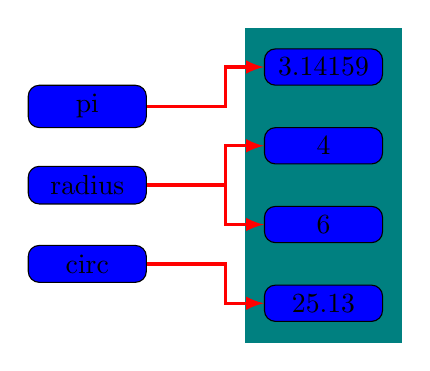
\begin{tikzpicture}[
				label/.style={rounded corners, draw=black, fill=Blue, text=black, minimum width=1.5cm}
				]
				\fill[Teal] (0,0) rectangle + (2,4);
				\node<1->[label](pinum) at (1,3.5) {3.14159};
				\node<2->[label](radnum) at (1,2.5) {4};
				\node<4->[label](radnum2) at (1,1.5) {6};
				\node<3->[label](circnum) at (1,0.5) {25.13};

				\node<1->[label](pi) at (-2,3) {pi};
				\node<2->[label](rad) at (-2,2) {radius};
				\node<3->[label](circ) at (-2,1) {circ};

				\draw<1->[Red, very thick, -latex] (pi.east) -- +(1,0) |- (pinum.west);
				\draw<2-3>[Red, very thick, -latex] (rad.east) -- +(1,0) |- (radnum.west);
				\draw<4->[Red, very thick, -latex] (rad.east) -- +(1,0) |- (radnum2.west);
				\draw<3->[Red, very thick, -latex] (circ.east) -- +(1,0) |- (circnum.west);

			\end{tikzpicture}
		\end{center}
	\end{columns}
\end{frame}

\begin{frame}{Variable Names}
	There are some important things to keep in mind when coming up with variable names:
	\begin{itemize}
		\item Capitalization matters! \pyi{radius} and \pyi{Radius} are different
		\item Variables can have numbers in the name, but they can't \emph{start} with a number
		\item Underscores are the only acceptable special character
		\item There is a small set of special python keywords that you can't use for variables.
			\begin{itemize}
				\item My general recommendation is, if the name gets highlighted when you type it because the IDE thinks it is important, choose a different name
			\end{itemize}
		\item \textcolor{Red}{Make your variable names meaningful!}
	\end{itemize}
\end{frame}

%\begin{frame}[fragile]{Two other \#Comments}
	%\vspace{5mm}
	%\begin{itemize}
		%\item You can assign multiple variables at the same time
			%\begin{pythoncode}
				%x, y = 5, 10	
			%\end{pythoncode}
			%\begin{itemize}
				%\item This can be useful for swapping variables, since everything gets evaulated before the bindings are assigned
					%\begin{pythoncode}
						%x, y = y, x
					%\end{pythoncode}
			%\end{itemize}
		%\item Use comments in your code to explain otherwise confusing or unclear sections
			%\begin{pythoncode}
				%#This is a comment
				%#The interpreter will completely ignore these
				%#lines while the code is being executed
				%4 + 5
			%\end{pythoncode}
	%\end{itemize}
%\end{frame}

%\begin{frame}[fragile]{Understanding Check}
	%What is the final printed value of \pyi{A} in the code below?
	%\begin{pythoncode}[numbers=left]
		%A = 10
		%B = 5
		%C = A * B
		%A = C - A
		%A, B, C = C, A, B
	%\end{pythoncode}
	%\begin{poll}
	%\item 10
	%\item \alert<2>{50}
	%\item 40
	%\item 200
	%\end{poll}
%\end{frame}

%\begin{frame}{Enter the Arena}
	%You have some options in what environment you'd like to write your code:
	%\begin{columns}
		%\column{0.5\textwidth}
		%\only<1>{
			%\begin{itemize}
				%\item Spyder
					%\begin{itemize}
						%\item Default python IDE
						%\item Lots of buttons and menus
						%\item Variable explorer can be useful
					%\end{itemize}
			%\end{itemize}
		%}
		%\only<2>{
			%\begin{center}
				%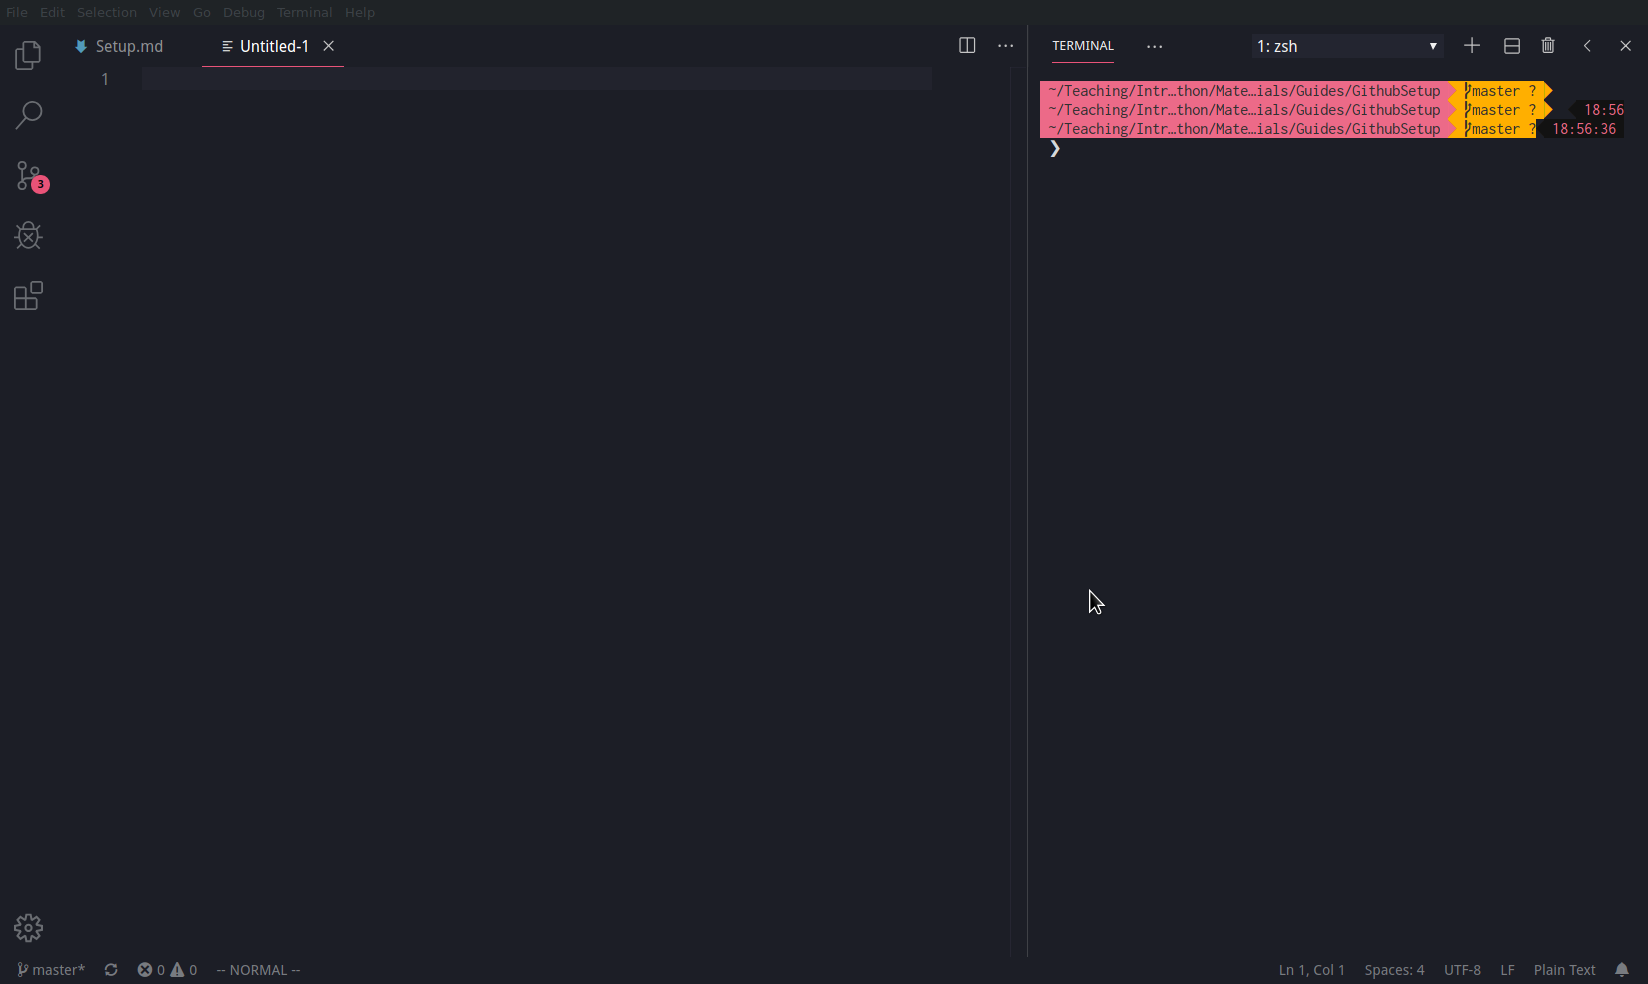
\includegraphics[width=\textwidth]{VSCodeScreen.png}
			%\end{center}
		%}
		%\column{0.5\textwidth}
		%\only<1>{
			%\begin{center}
				%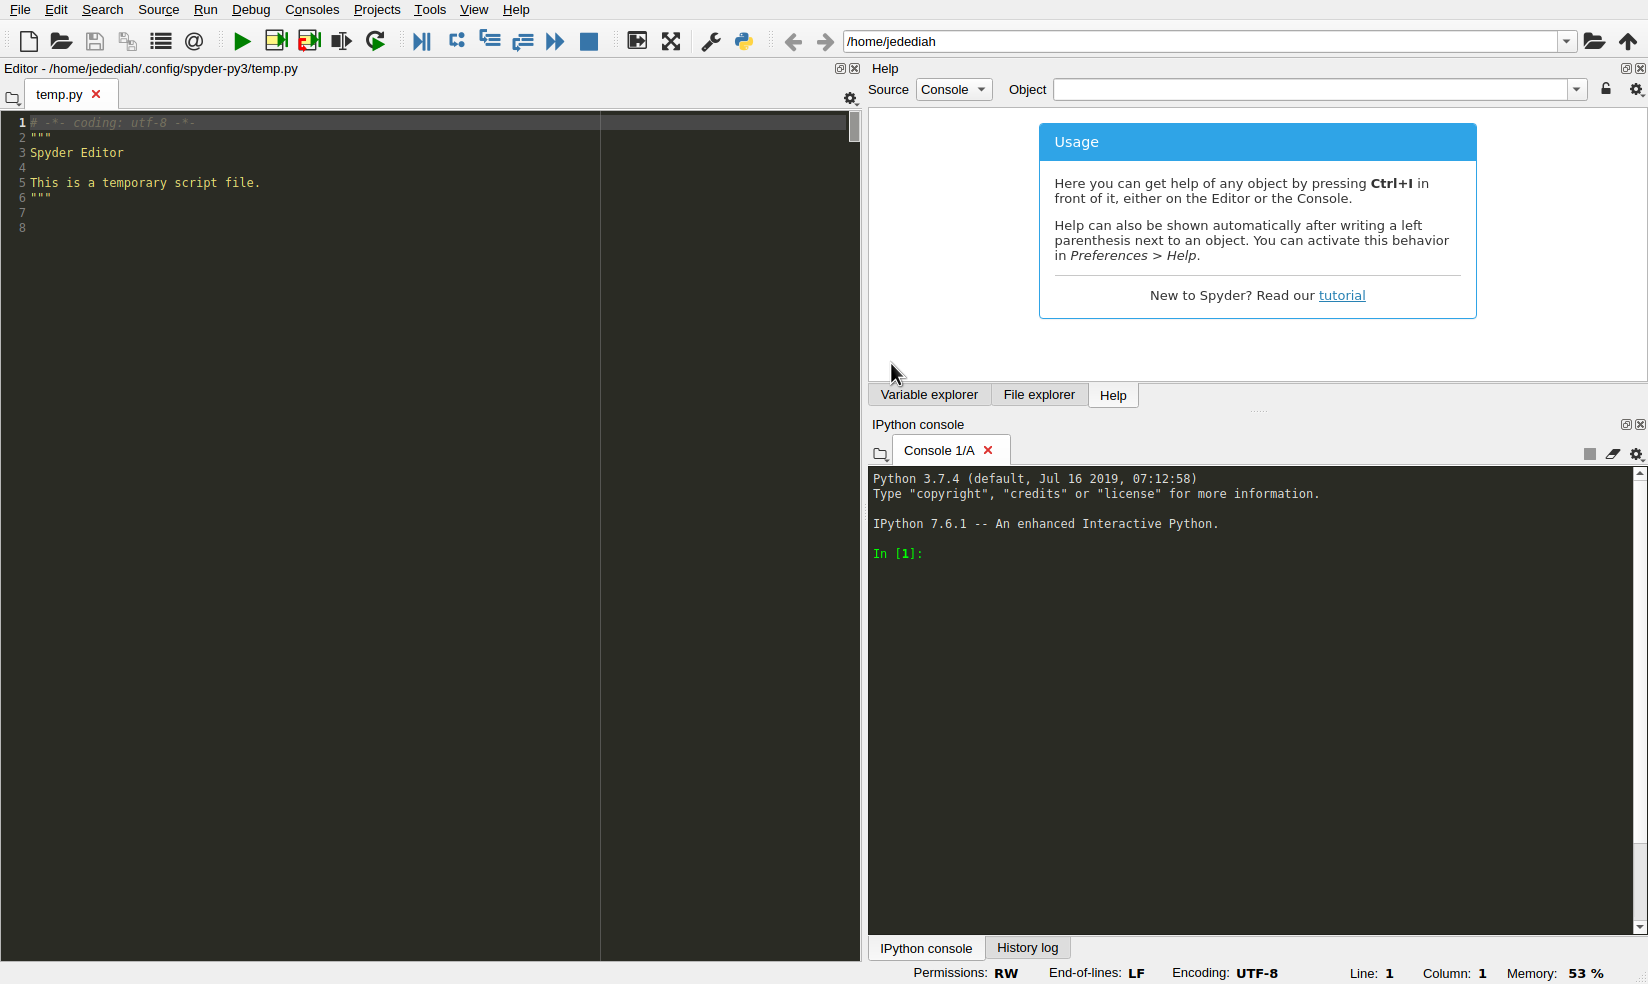
\includegraphics[width=\textwidth]{SpyderScreen.png}
			%\end{center}
		%}
		%\only<2>{
			%\begin{itemize}
				%\item VSCode
					%\begin{itemize}
						%\item More modern design and quite popular
						%\item More minimal in presentation 
						%\item Huge extension functionality
					%\end{itemize}
			%\end{itemize}
		%}
		
	%\end{columns}
%\end{frame}





\end{document}

